\section{Introduction}
\label{sec:introduction}

% state the learning objective 
With this project, we aimed to better understand RC circuits, and study how they respond under various scenarios. In order to achieve our goals, we focused our attention in the circuit shown bellow

\begin{figure}[h] \centering
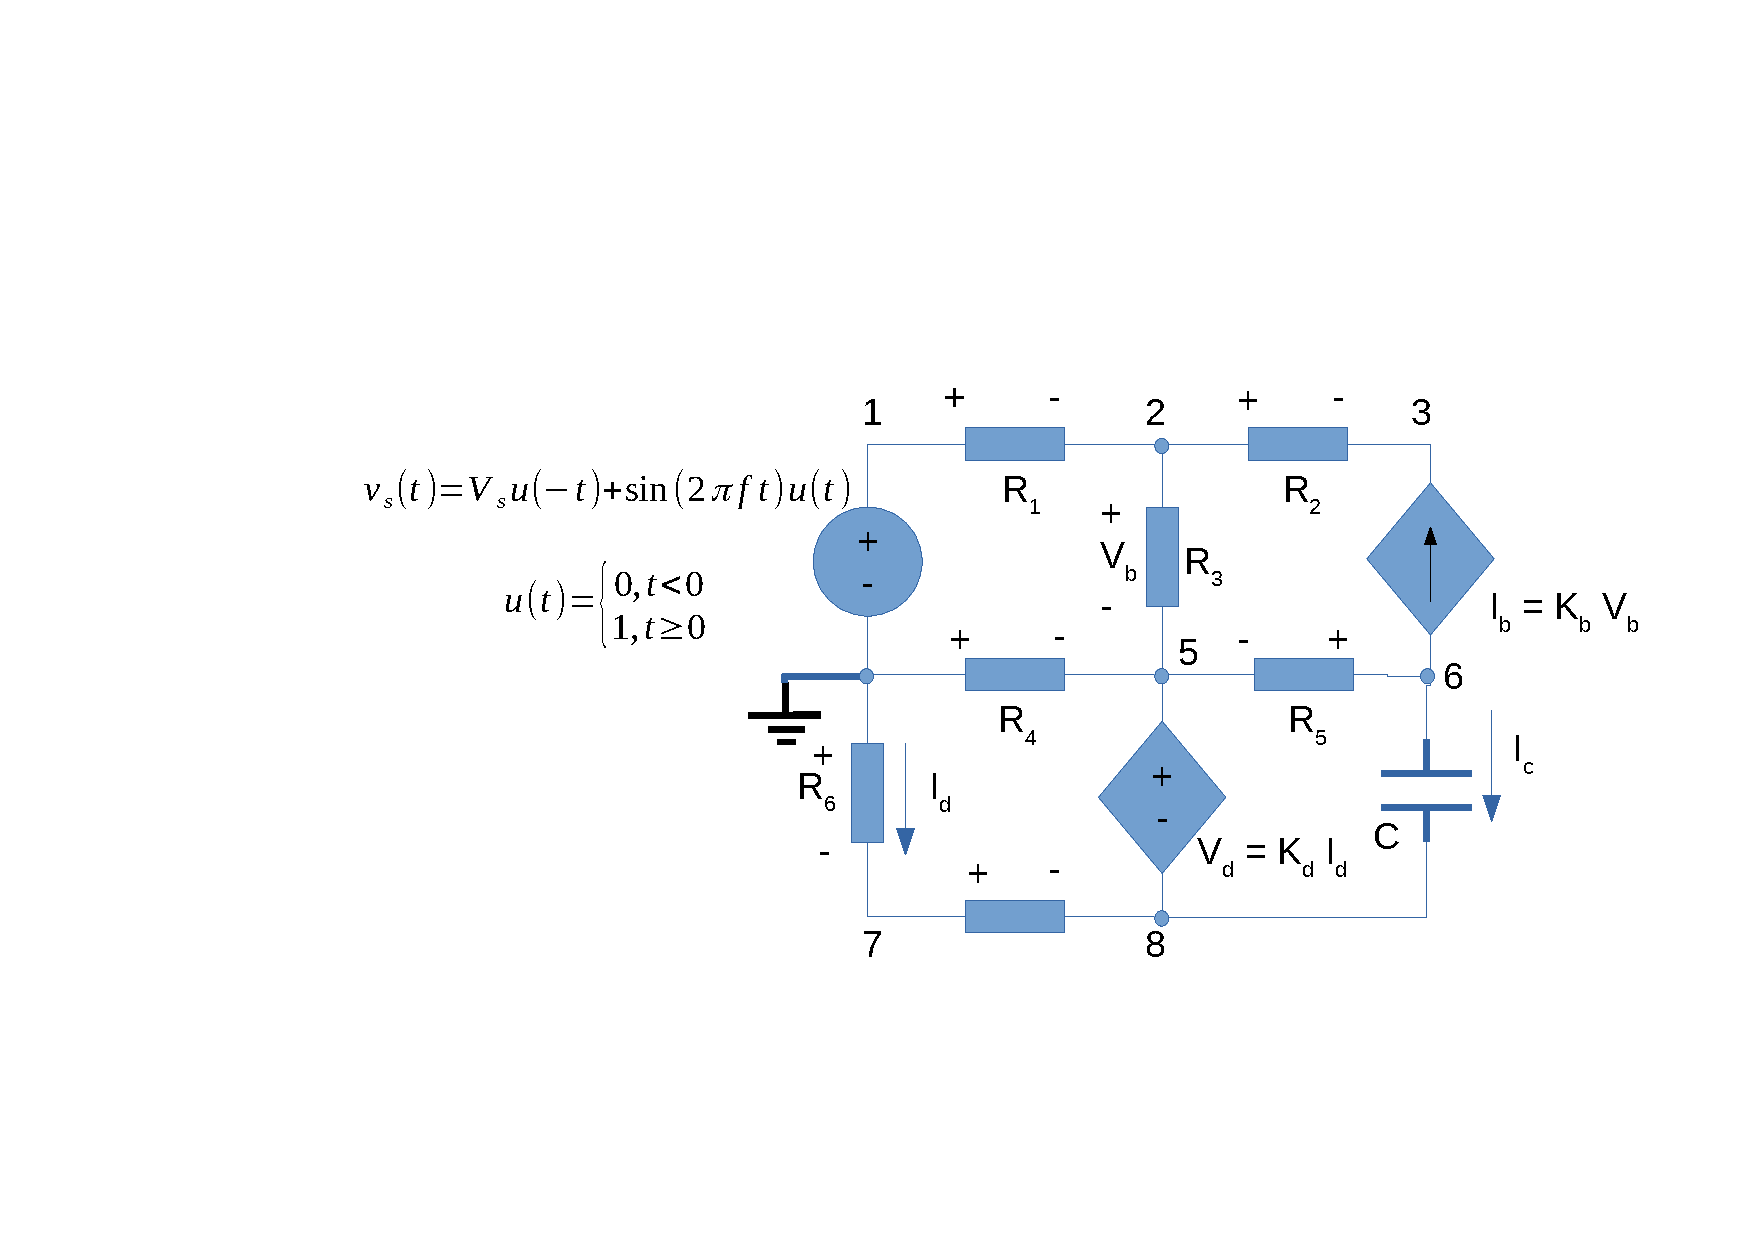
\includegraphics[width=0.4\linewidth]{Circuito.pdf}
\caption{Studied Circuit.}
\label{fig:rc}
\end{figure}

We then began by analysing the circuit by the now familiar nodal analysis method and compared it to the results obtained with the software \textit{ngspice}, when the voltage source outputted a constant voltage. Following that, we than turned our attention, to analysing the system under a sinusoidal voltage input. Thus the system was studied at the instant where the voltage was changed, and then the general response of the system was obtained both theoretically and through simulations, by adding the natural and forced solution of the system for a given driving frequency. At last, we concluded our survey, by examining the response of the system for a wide range of driving frequencies, and plotting both the magnitude and phase of the voltages obtained at the terminals of the capacitor. At every step, the theoretical results were compared with the data obtained from simulating the circuit.  

